\chapter{Green Function Technique}
	Now, we would solve the wave equations 1.5 and 1.6 using a technique known as the Green Function Technique. The Green function technique is applied in solving inhomogeneous ordinary differential equation which, in this case, is what we have. The Green function technique solves for the Green function, which is a scalar denoted by G for the differential equation given. The Green function, G is the impulse response of the differential equation. For the wave equation, G is the spatial impulse response of the system which is described by the wave equation. 
	$$\nabla^{2}\bar{A}-\mu\bar{A} = -\mu\bar{J};$$
	Let us note that the Laplace operator is a scalar operator (it operates on a scalar) which means it operates on each component of the $\bar{A}$ vector. So essentially replacing the vector $\bar{A}$ with a scalar is possible.
	Points to note when using the technique:
	\begin{itemize}
		\item First, we replace in the differential equation, the original function (in this case, $\bar{A}$ and V) with the Green function and replace the driving quantity (in this case $-\mu\bar{J}$ and $-\frac{\rho}{\epsilon}$) with the impulse function $\delta = f_{n}$(space).
		\item Next, we convolve the solution of the Green function with the driving quantity to get the solution to the original function.
	\end{itemize}
	\par Before applying the Green function technique, we know that the fields $\vec{E}$ $\vec{H}$ are time-varying fields and so, $\vec{A}$ is also a time-varying field and vary with respect to $e^{j\omega t}$, hence,
	$$\frac{\partial}{\partial t} \equiv j\omega $$ and  $$\frac{\partial^{2}}{\partial t^{2}} \equiv j\omega.j\omega = -\omega^{2}$$
	
	
	Therefore, the equation is rewritten as:
	$$\nabla^{2}\bar{A}-\omega^{2}\mu\bar{A} = -\mu\bar{J},$$ recall from the wave equation, in an inbound medium,
	$$\beta^{2} = \omega^{2}\mu \varepsilon;$$
	$$\beta = \omega\sqrt{\mu \varepsilon}$$
	$$  \beta    = \omega\sqrt{\mu_o \varepsilon_o} \ for \ free  \ space$$
	So,
	$$\nabla^{2}\bar{A}+\beta^{2}\bar{A} = -\mu\bar{J}$$
	Applying Green function technique, then,
	$$\nabla^{2}\bar{G}+\beta^{2}\bar{G} = \delta(space)$$
	Solving the equation in the spherical coordinate system,
	$$\frac{\partial}{\partial r} (r^{2} \frac{\partial G}{\partial r} ) + \frac{1}{r^2 \sin \theta} \frac{\partial}{\partial  \theta}(\sin \theta \frac{\partial G}{\partial \theta}) + \frac{1}{r^{2}\sin^{2}\theta} \frac{\partial^{2}}{\partial\phi^{2}} + \beta^{2}G = \delta(r,\theta,\phi)$$
	\par Considering the source at the origin (impulse located at origin) simplifies the solution because at whatever direction in space , you see the same source which make solution for the equation spherically symmetric. Hence, G is not function of $\theta$ and $\phi$
	 $$\frac{\delta}{\delta \theta} \equiv \frac{\delta}{\delta \phi} = 0$$
	 \begin{equation}
	      	\frac{d}{d r}(r^{2}\frac{d G}{d r}) +  \beta^{2}G = \delta(r)
	 \end{equation}

	\par Notice the partial derivatives is converted to full derivatives because $G = f_{n}(r)$ only.\\
	\par Let's define a variable $\psi = rG$
	$$\frac{d\psi}{dr} = r\frac{dG}{dr} + G \Longrightarrow \frac{dG}{dr} = \frac{1}{r}{\frac{d\psi}{dr} - G}$$

	and $G = \frac{\psi}{r}$ substitute in equation 2.1
	
	$$\frac{1}{r^{2}}\frac{d}{dr}[r^{2}
	[\frac{1}{r}(\frac{d\psi}{dr} - G)]] + \beta^{2}\frac{\psi}{r} = \delta(r)$$
	
	$$\frac{1}{r^{2}}\frac{d}{dr}[r\frac{d\psi}{dr} - rG] + \beta^{2}\frac{\psi}{r} = \delta(r)$$
	
	$$\frac{1}{r^{2}}\frac{d}{dr}[r\frac{d\psi}{dr}] - \frac{1}{r^{2}}\frac{d}{dr}(rG) + \beta^{2}\frac{\psi}{r} = \delta(r)$$
	
	$$\frac{1}{r^{2}}[r\frac{d^{2}\psi}{dr^{2}} + \frac{d\psi}{dr}] - \frac{1}{r^{2}}\frac{d\psi}{dr} + \beta^{2}\frac{\psi}{r} = \delta(r)$$
	$$\frac{1}{r}\frac{d^{2}\psi}{dr^{2}} + \frac{1}{r^{2}}\frac{d\psi}{dr} - \frac{1}{r^{2}}\frac{d\psi}{dr} + \beta^{2}\frac{\psi}{r} = \delta(r)$$
	
	$$\frac{1}{r}[\frac{d^{2}\psi}{dr^{2}} + \beta^{2}\psi] = \delta(r)$$
	
	$$\frac{d^{2}\psi}{dr^{2}} + \beta^{2}\psi = \delta(r)$$
	which has the solution $\psi = Ce^{-j\beta r} + De^{j\beta r}$. The two terms represent the travelling waves in the direction of r and r is always positive in the spherical  coordinate system. The first term represents a wave which is travelling in all positive direction, ie away from the origin, while the second term represents a wave which is travelling in the negative r direction but r is always positive, so it represents a wave that is moving towards the origin. Since our source is at the origin and there is no energy source elsewhere in the medium, then this wave does not exist. The solution now reduces to:
	$\psi = Ce^{-j\beta r}$ and $\psi = Gr; G = \frac{\psi}{r}$
	$G = \frac{Ce^{-j\beta r}}{r}$
	\begin{figure}[h]
		\vspace{-20pt}
		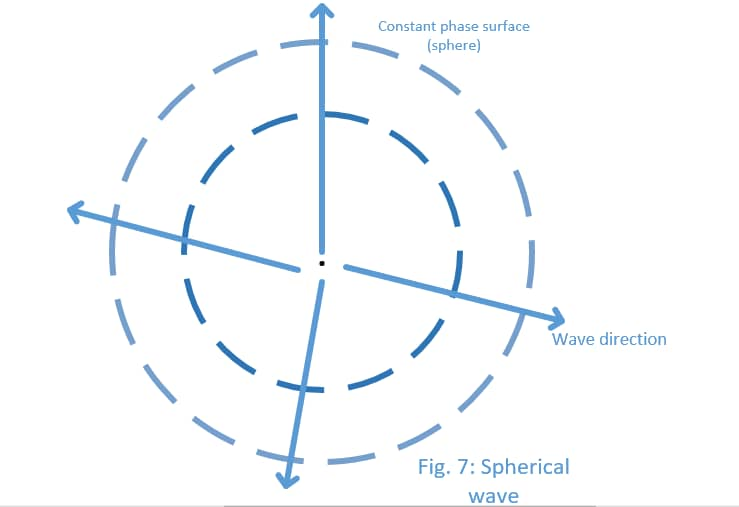
\includegraphics[width=\linewidth]{img_1}
		\centering
		\caption{Spherical wave}
		\label{fig:1}
	\end{figure}
	It should be noted that a constant r represents the constant phase surface. In the spherical coordinate system when r equals a constant, we know it represents a sphere so these constant phase surfaces are spheres and the wave propagating is called the spherical wave. Also, one other thing to be noted is that the amplitude of the spherical wave reduces as $\frac{1}{r}$ as opposed to the uniform  plane wave in which the amplitude does not change as a function of time.\\
	In conclusion, the solution of the Green function, G gives a spherical wave whose  reduces as  $\frac{1}{r}$ and whose phase fronts are spheres.\\
	But the solution is not complete as the solution of the Green function is the impulse response which is the complementary solution  of the differential equation, hence, let's compute C by applying the appropriate boundary conditions.\\
	To evaluate C, we substitute the general solution of $G = \frac{Ce^{-j\beta r}}{r}$ in the original differential equation in equation 2.1, integrate the whole expression over the volume around the origin and then take a limit when $r\rightarrow0$
	\begin{dmath*}
		\lim\limits_{r\rightarrow0} \int_{0}^{r} \int_{0}^{\pi}\int_{0}^{2\pi}\frac{1}{r^{2}}\frac{d}{dr}\left[{r^{2}}\frac{d}{dr}\left[\frac{Ce^{-j\beta r}}{r}\right]\right]r^{2}\sin\theta dr d\theta d\phi + \beta^{2} \int_{0}^{r} \int_{0}^{\pi}\int_{0}^{2\pi}\frac{Ce^{-j\beta r}}{r}r^{2}\sin\theta drd\theta d\phi
	\end{dmath*}
	
	$$= \int_{v}\delta(r)dr$$
	
	\begin{dmath*}
		\lim\limits_{r\rightarrow0} \int_{0}^{r} \int_{0}^{\pi}(2\pi)\frac{d}{dr}\left[{r^{2}}\frac{d}{dr}\left[\frac{Ce^{-j\beta r}}{r}\right]\right]\sin\theta d\theta dr + \beta^{2} \int_{0}^{r} \int_{0}^{\pi}(2\pi)\sin\theta d\theta[rCe^{-j\beta r}]dr = \int_{v}\delta(r)dr
	\end{dmath*}
	
	\begin{dmath*}
		\lim\limits_{r\rightarrow0} \left[4\pi\int_{0}^{r}\frac{d}{dr}\left[{r^{2}}\frac{d}{dr}\left[\frac{Ce^{-j\beta r}}{r}\right]\right]dr + C\beta^{2}4\pi\int_{0}^{r}re^{-j\beta r}dr\right] = \int_{v}\delta(r)dr
	\end{dmath*}

	\begin{dmath*}
		\lim\limits_{r\rightarrow0} \left[4\pi\int_{0}^{r}\frac{d}{dr}\left[{Cr^{2}}\left[\frac{r(-j\beta e^{-j\beta r}) - e^{-j\beta r}}{r^{2}}\right]\right]dr + C\beta^{2}4\pi\int_{0}^{r}re^{-j\beta r}dr\right] = \int_{v}\delta(r)dr
	\end{dmath*}
	
	\begin{dmath*}
		\lim\limits_{r\rightarrow0} \left[4\pi\int_{0}^{r}\frac{d}{dr}\left[{Cr^{2}}\left[\frac{-jr\beta e^{-j\beta r} - e^{-j\beta r}}{r^{2}}\right]\right]dr + C\beta^{2}4\pi\int_{0}^{r}re^{-j\beta r}dr\right] = \int_{v}\delta(r)dr
	\end{dmath*}
	
	\begin{dmath*}
		\lim\limits_{r\rightarrow0} \left[4\pi\int_{0}^{r}\frac{d}{dr}\left[{-Cr^{2}} e^{-j\beta r}\left(\frac{jr\beta+1}{r^{2}}\right)\right]dr + C\beta^{2}4\pi\int_{0}^{r}re^{-j\beta r}dr\right] = \int_{v}\delta(r)dr
	\end{dmath*}
	
	\begin{dmath*}
		\lim\limits_{r\rightarrow0} \left[4\pi\int_{0}^{r}\frac{d}{dr}\left(-[{C} e^{-j\beta r}(jr\beta+1)]\right)dr + C\beta^{2}4\pi\int_{0}^{r}re^{-j\beta r}dr\right] = \int_{v}\delta(r)dr
	\end{dmath*}

	\begin{dmath*}
		\lim\limits_{r\rightarrow0} \left[4\pi\int_{0}^{r}\left[-[{C} e^{-j\beta r}(j\beta) + (jr\beta+1)(-j\beta e^{-j\beta r})]\right]dr + C\beta^{2}4\pi\int_{0}^{r}re^{-j\beta r}dr\right] = \int_{v}\delta(r)dr
	\end{dmath*}
	
	\begin{dmath*}
		\lim\limits_{r\rightarrow0} \left[4\pi\int_{0}^{r}-C[j\beta e^{-j\beta r}-j\beta(jr\beta+1)e^{-j\beta r}]dr + C\beta^{2}4\pi\int_{0}^{r}re^{-j\beta r}dr\right] = \int_{v}\delta(r)dr
	\end{dmath*}

	\begin{dmath*}
		\lim\limits_{r\rightarrow0} \left[4\pi\int_{0}^{r}-jCe^{-j\beta r}(1-j\beta r-1)dr + C\beta^{2}4\pi\int_{0}^{r}re^{-j\beta r}dr\right] = \int_{v}\delta(r)dr
	\end{dmath*}
	
	\begin{dmath*}
		\lim\limits_{r\rightarrow0} \left[4\pi\int_{0}^{r}-C\beta^{2}re^{-j\beta r}dr + C\beta^{2}4\pi\int_{0}^{r}re^{-j\beta r}dr\right] = \int_{v}\delta(r)dr
	\end{dmath*}
	
	\begin{dmath*}
		\lim\limits_{r\rightarrow0} \left[-C4\pi\beta^{2}\int_{0}^{r}re^{-j\beta r}dr + C\beta^{2}4\pi\int_{0}^{r}re^{-j\beta r}dr\right] = \int_{v}\delta(r)dr
	\end{dmath*}
	
	$$u = r;\ dv=e^{-j\beta r}dr;\ du=dr;\ v=j\frac{e^{-j\beta r}}{\beta}$$

	\begin{dmath*}
		\lim\limits_{r\rightarrow0} \left[-C4\pi\beta^{2}\left[j\frac{re^{-j\beta r}}{\beta}\bigg\vert_{0}^{r}\frac{-j}{\beta}\int_{0}^{r}e^{-j\beta r}dr\right] + C\beta^{2}4\pi\int_{0}^{r}re^{-j\beta r}dr\right] = \int_{v}\delta(r)dr
	\end{dmath*}
	
	\begin{dmath*}
		\lim\limits_{r\rightarrow0} \left[-C4\pi\beta^{2}\left[j\frac{re^{-j\beta r}}{\beta}  \frac{-j}{\beta}\left(j\frac{e^{-j\beta r}}{\beta}\right)\right] + C\beta^{2}4\pi\int_{0}^{r}re^{-j\beta r}dr\right] = \int_{v}\delta(r)dr
	\end{dmath*}
	
	\begin{dmath*}
		\lim\limits_{r\rightarrow0} \left[-C4\pi\beta^{2}\left[j\frac{re^{-j\beta r}}{\beta}  +\frac{e^{-j\beta r}}{\beta^{2}}\right] + C\beta^{2}4\pi\int_{0}^{r}re^{-j\beta r}dr\right] = \int_{v}\delta(r)dr
	\end{dmath*}

	\begin{dmath*}
		\lim\limits_{r\rightarrow0} \left[-C4\pi e^{-j\beta r}\left[j\frac{r\beta^{2}}{\beta} +\frac{\beta^{2}}{\beta^{2}}\right] + C\beta^{2}4\pi\int_{0}^{r}re^{-j\beta r}dr\right] = \int_{v}\delta(r)dr
	\end{dmath*}
	
	\begin{dmath*}
		\lim\limits_{r\rightarrow0} \left[-C4\pi e^{-j\beta r}(j\beta r+1) + C\beta^{2}4\pi\int_{0}^{r}re^{-j\beta r}dr\right] = \int_{v}\delta(r)dr
	\end{dmath*}
	
	By definition, the integral of delta function over a volume which encloses the delta function is 1.
	$$\lim\limits_{r\rightarrow0} \left[-C4\pi e^{-j\beta r}(j\beta r+1) + C\beta^{2}4\pi\int_{0}^{r}re^{-j\beta r}dr\right] = 1$$
	
	Taking limit $r\rightarrow0$ gives
	$$-4\pi C= 1$$
	
	$$C = \frac{-1}{4\pi}$$
	
	Hence, the complementary solution of the Green function is given as $ G= -\frac{e^{-j\beta r}}{4\pi r}$
	With the impulse response, G we can find the solution to $\vec{A}$ which is the convolution of the impulse response with the driving function.\\
	Hence, 
	\begin{equation}
	     \vec{A}=\int_{v}\mu\vec{J}(r^{'}) \frac{e^{-j\beta\vert\vec{r}-\vec{r^{'}}\vert}}{4\pi|\vec{r}-\vec{r^{'}}|}dV'
	\end{equation}
	
	which is the convolution integral. $\vec{r^{'}}$ denotes the position vector of the location of the current, while r is the position vector of the location where we are computing the vector potential. The expression can be best understood by considering figure 2.2, where there is a region where the source is located, denoted by $\vec{J}(r')$, for an infinitesimal volume, $dV^{'}$, the current is given by $\vec{J}(r')dV$. Also, there is one observation point where the vector potential is to be determined. The contribution of vector potential, dA from the infinitesimal volume is given by: 
	\begin{equation}
		\mu\vec{J}(r^{'}) \frac{e^{-j\beta|\vec{r}-\vec{r^{'}}|}}{4\pi|\vec{r}-\vec{r^{'}}|}dV',
	\end{equation}
so integrating it over the region of the space where the source is, gives the total vector potential given by equation 2.2.
		\begin{figure}[H]
		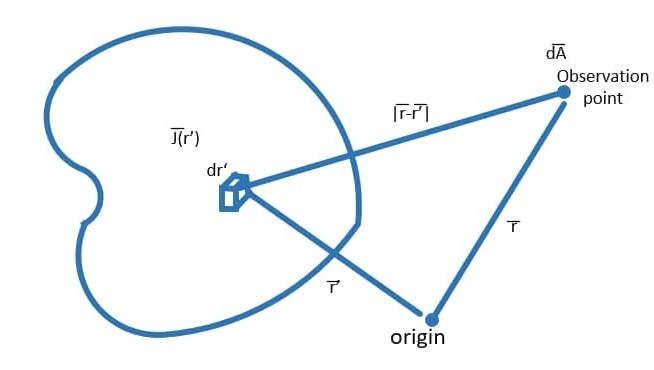
\includegraphics[width=1\linewidth]{img_2}
		\centering
		\caption{}
		\label{fig:1}
		\vspace{-10pt}
	\end{figure}\newline
	The reason for the mod sign in the equation 2.2 is to always have a positive value of r.\\
	So with the current distribution at the location $\vec{r^{'}}$, the magnetic vector potential at any point $\vec{r}$ can be calculated.\\
	\par In this course, when modelling antennas, we assume the current distribution is given prior to the problem and our solution is simplified to just solving for the fields. However, if the current distribution were not given, then with some excitation point on the structure, the solution to the problem can be gotten from Maxwell's equation. But like it was said earlier, the current distribution is assumed to be given.